\documentclass[11pt,answers]{exam}

\usepackage{etex}
\usepackage{amssymb,amsmath,multicol} %<-- InWorksheetExam1 i also have fancyhdr,

\usepackage[metapost]{mfpic}
\usepackage[pdftex]{graphicx}
\usepackage{tabu}

\usepackage{pst-plot}
\usepackage{pgfplots}
\pgfplotsset{compat=1.9}

\usepackage{tikz}
\usepackage{tkz-2d}
\usepackage{tkz-base}
\usetikzlibrary{calc}
\usetikzlibrary{arrows}

\usepackage{systeme}

\usepackage[inline]{enumitem}
\usepackage{refcount}%<-- non in WorksheetExam1

\usepackage{pstricks-add,pst-eucl}
\usepackage{systeme}
\usepackage{setspace}
\usepackage{multicol}


\usepackage[inline]{enumitem}   
\makeatletter
% This command ignores the optional argument for itemize and enumerate lists
\newcommand{\inlineitem}[1][]{%
\ifnum\enit@type=\tw@
    {\descriptionlabel{#1}}
  \hspace{\labelsep}%
\else
  \ifnum\enit@type=\z@
       \refstepcounter{\@listctr}\fi
    \quad\@itemlabel\hspace{\labelsep}%
\fi}
\makeatother


\def\f{x+1} \def\g{-x/3+2}  \def\h{-x+3}

\newcommand{\vasymptote}[2][]{
    \draw [densely dashed,#1] ({rel axis cs:0,0} -| {axis cs:#2,0}) -- ({rel axis cs:0,1} -| {axis cs:#2,0});
}

\boxedpoints

\addpoints
%\printanswers
\noprintanswers

\opengraphsfile{Q9a_Fa18}

\begin{document}
\extrawidth{-0.3in}
\pagestyle{headandfoot}

\setlength{\hoffset}{-.25in}

\extraheadheight{-.3in}
\runningheadrule
\firstpageheader{\bfseries {Precalculus}}{ \bfseries {Quiz 10 }}{\bfseries {11/27/18}} 

\begin{center}
	This quiz has \numquestions\ questions, for a total of \numpoints\
	points and \numbonuspoints\ bonus points.
\end{center}


\firstpagefooter{} %%&&CHANGED
                {}
                {%Points earned: \hbox to 0.5in{\hrulefill}
                % out of  \pointsonpage{\thepage} points
                }
                 
						

\vspace*{0.1cm}
\hbox to \textwidth { \scshape {Name:} \enspace\hrulefill}
\vspace{0.1cm}




\pointpoints{point}{points}

\begin{questions}


\addpoints


\question Identify the quadrant of the unit circle that contains the terminal point of each of the numbers listed below.
\bigskip


\begin{parts}
	\part[1] $\displaystyle t=-\frac{3\pi}{4}$
	
	%\begin{multicols}{2}	
	\begin{oneparchoices}
		\choice Top right quadrant; \choice Top left quadrant;
		\choice Bottom right quadrant; \choice Bottom left quadrant. 
	\end{oneparchoices}
	
	\part[1] $\displaystyle t=1$
	
	%\begin{multicols}{2}	
	\begin{oneparchoices}
		\choice Top right quadrant; \choice Top left quadrant;
		\choice Bottom right quadrant; \choice Bottom left quadrant. 
	\end{oneparchoices}
	%\end{multicols}	
	
	
	
	
\end{parts}
\bigskip

\question Find the period of each of the functions listed below:
\bigskip

\begin{parts}
	\part[1] $\displaystyle y=4\sin(4x)$ \dotfill
	\part[1] $\displaystyle y=4\sin(x)+4$ \dotfill
	\part[1] $\displaystyle y=0.4\sin\left (\frac{x}{4}\right )$ \dotfill
\end{parts}

%\question[1] Find $\displaystyle g\left(\frac{11\pi}{12}\right)$, where $\displaystyle g(t)=2\cos\left (t+\frac{\pi}{12}\right)$. 

\bigskip

%\dotfill

\question Find the exact value of each of the following:
\bigskip

\begin{parts}
	\part[1] $\displaystyle \sin\left(\frac{49\pi}{3}\right)$ \dotfill
	\part[1] $\displaystyle \cos\left(\frac{49\pi}{3}\right)$ \dotfill
	\bonuspart[1] $\displaystyle \sin\left( -\frac{5\pi}{3} \right)$ \dotfill
\end{parts}	

\question A Ferris wheel with 59 capsules has a diameter of 110 meters and its lowest point (at the 6 o'clock position) is 5 meters above the ground. One full rotation of the wheel takes 24 minutes, and the wheel rotates counterclockwise at a constant speed. The capsules are labeled from 1 to 59. We start observing when capsule 1 is at the lowest point on the wheel. If $H(t)$ is the height of capsule 1 $t$ minutes after we start the observation, then: 

\bigskip

\begin{parts}
	\part[1] The equation of the midline of $H(t)$ is:
	\begin{oneparchoices}
		\choice $y=5$; \choice $y=24$;  \choice $y=55$; \choice $y=60$; \choice $y=110$; \choice $y=115$. 
	\end{oneparchoices}
	
	\part[1] The amplitude of $H(t)$ is:
	
	\begin{oneparchoices}
		\choice 5; \choice 24; \choice 55; \choice 60; \choice 110;  \choice 115.
	\end{oneparchoices}
	
	
	
	
	
	
	
\end{parts}

\end{questions}
\newpage

\par\medskip\hrule\medskip


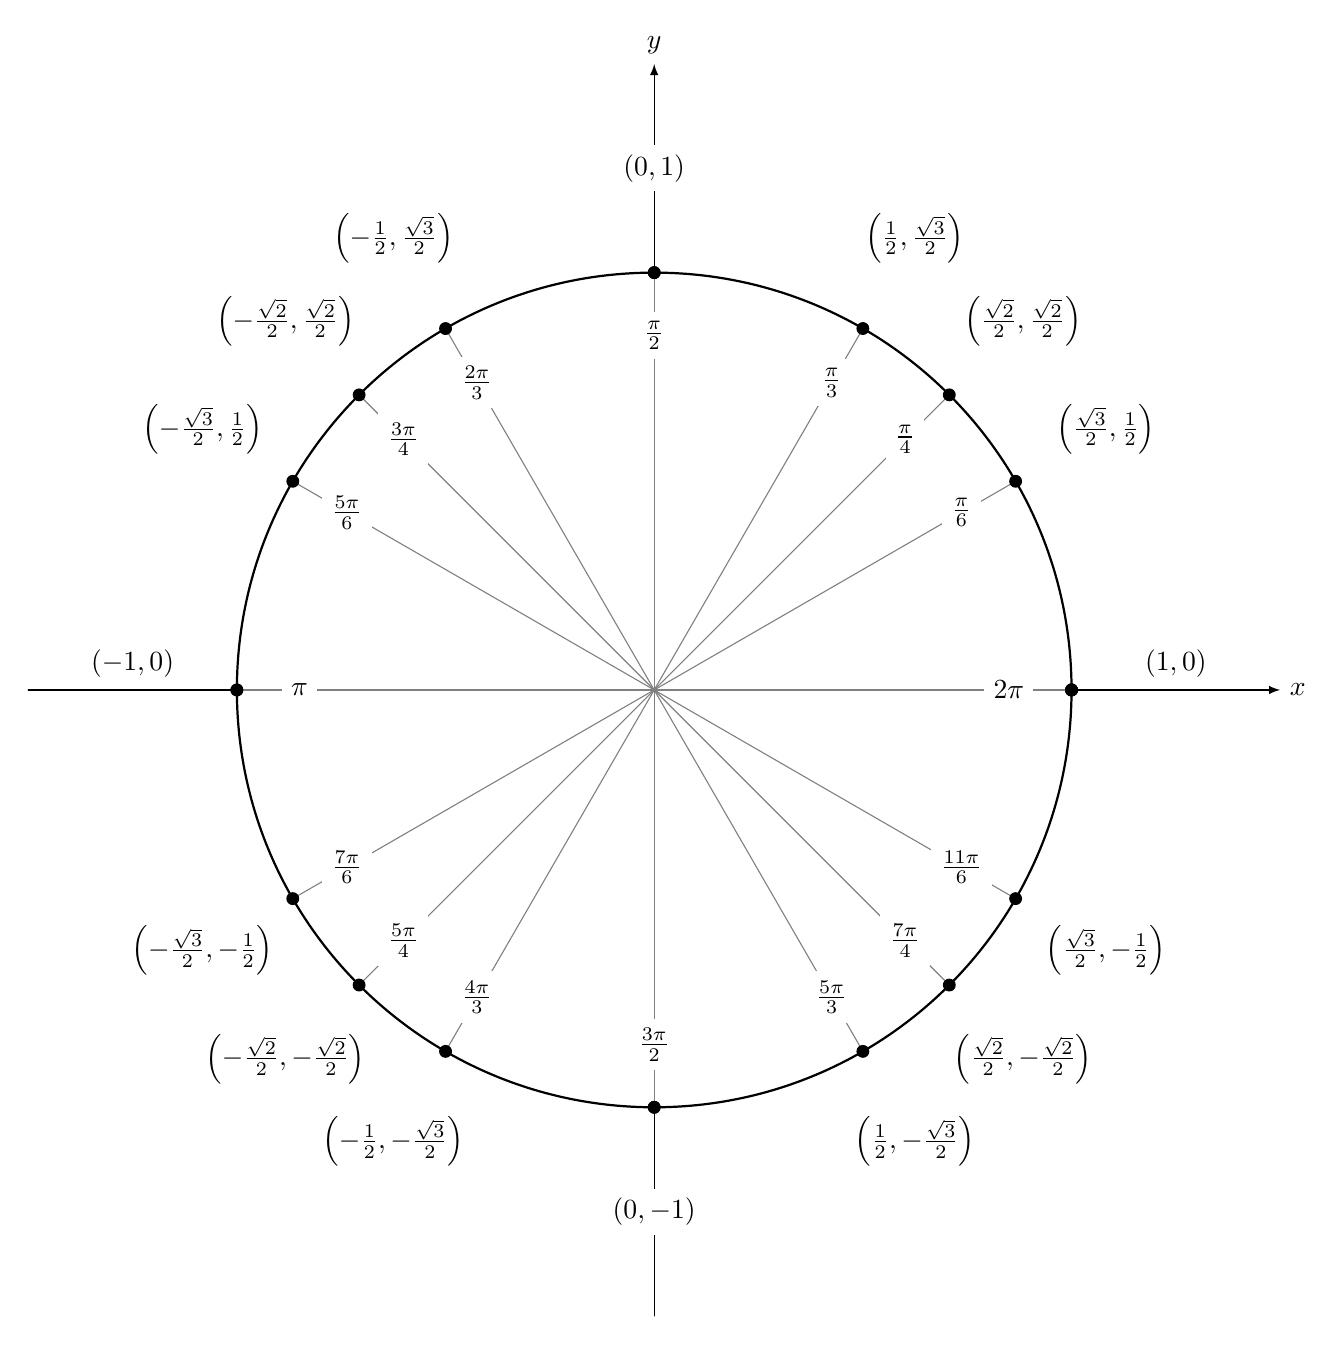
\begin{tikzpicture}[scale=5.3,cap=round,>=latex]
% draw the coordinates
\draw[->] (-1.5cm,0cm) -- (1.5cm,0cm) node[right,fill=white] {$x$};
\draw[->] (0cm,-1.5cm) -- (0cm,1.5cm) node[above,fill=white] {$y$};

% draw the unit circle
\draw[thick] (0cm,0cm) circle(1cm);

\foreach \x in {0,30,...,360} {
	% lines from center to point
	\draw[gray] (0cm,0cm) -- (\x:1cm);
	% dots at each point
	\filldraw[black] (\x:1cm) circle(0.4pt);
	% draw each angle in degrees
	%\draw (\x:0.6cm) node[fill=white] {$\x^\circ$};
}

\foreach \x in {0,45,...,360} {
	% lines from center to point
	\draw[gray] (0cm,0cm) -- (\x:1cm);
	% dots at each point
	\filldraw[black] (\x:1cm) circle(0.4pt);
	% draw each angle in degrees
	%\draw (\x:0.6cm) node[fill=white] {$\x^\circ$};
}
% draw each angle in radians
\foreach \x/\xtext in {
	30/\frac{\pi}{6},
	45/\frac{\pi}{4},
	60/\frac{\pi}{3},
	90/\frac{\pi}{2},
	120/\frac{2\pi}{3},
	135/\frac{3\pi}{4},
	150/\frac{5\pi}{6},
	180/\pi,
	210/\frac{7\pi}{6},
	225/\frac{5\pi}{4},
	240/\frac{4\pi}{3},
	270/\frac{3\pi}{2},
	300/\frac{5\pi}{3},
	315/\frac{7\pi}{4},
	330/\frac{11\pi}{6},
	360/2\pi}
\draw (\x:0.85cm) node[fill=white] {$\xtext$};

\foreach \x/\xtext/\y in {
	% the coordinates for the first quadrant
	30/\frac{\sqrt{3}}{2}/\frac{1}{2},
	45/\frac{\sqrt{2}}{2}/\frac{\sqrt{2}}{2},
	60/\frac{1}{2}/\frac{\sqrt{3}}{2},
	% the coordinates for the second quadrant
	150/-\frac{\sqrt{3}}{2}/\frac{1}{2},
	135/-\frac{\sqrt{2}}{2}/\frac{\sqrt{2}}{2},
	120/-\frac{1}{2}/\frac{\sqrt{3}}{2},
	% the coordinates for the third quadrant
	210/-\frac{\sqrt{3}}{2}/-\frac{1}{2},
	225/-\frac{\sqrt{2}}{2}/-\frac{\sqrt{2}}{2},
	240/-\frac{1}{2}/-\frac{\sqrt{3}}{2},
	% the coordinates for the fourth quadrant
	330/\frac{\sqrt{3}}{2}/-\frac{1}{2},
	315/\frac{\sqrt{2}}{2}/-\frac{\sqrt{2}}{2},
	300/\frac{1}{2}/-\frac{\sqrt{3}}{2}}
\draw (\x:1.25cm) node[fill=white] {$\left(\xtext,\y\right)$};

% draw the horizontal and vertical coordinates
% the placement is better this way
\draw (-1.25cm,0cm) node[above=1pt] {$(-1,0)$}
(1.25cm,0cm)  node[above=1pt] {$(1,0)$}
(0cm,-1.25cm) node[fill=white] {$(0,-1)$}
(0cm,1.25cm)  node[fill=white] {$(0,1)$};
\end{tikzpicture}



\end{document}                 